\raggedright{}

\section{Abstract}\label{abstract}

This paper focuses on a historically understudied area in computing education: attending to students' \emph{design thinking} in university-level introductory programming courses. We offer an account of one student---``Rebecca''---and her experiences and code from a second-semester course on programming concepts for engineers. Using data from both code snapshots and clinical interviews, we explicate both the challenges of studying students' software design processes and the potential for such study to inform accounts of teaching and learning.We detail the case of Rebecca, a first-year Electrical Engineering student taking a required 2\textsuperscript{nd}-semester programming course in C. Our analysis focuses on two related aspects of Rebecca's code for a multi-week project:

\begin{enumerate}
\def\labelenumi{\arabic{enumi}.}
\tightlist
\item
  The origin, nature, and evolution of unusual structural and behavioral features of Rebecca's code
\item
  The subtle, yet complex reasons that led Rebecca to make particular design choices in her code
\end{enumerate}

Our data comes from ethnographic observation of Rebecca's class, fine-grained compile-time snapshots of Rebecca's codebase, and semistructured interviews with Rebecca. We first present an analysis of the compile-time snapshots, detailing Rebecca's unusual use of file-scanning loops and her seven-fold repetition of a particular code chunk (once for each day of the week). We then augment that analysis with data from semi-structured interviews with Rebecca, which reveal that affect \citep{hannula_affect_2004, eynde_case_2006} and framing \citep{vandesande_achieving_2012, hammer_resources_2005} offer substantial explanatory power for understanding why Rebecca made particular design choices.

\section{Introduction}\label{introduction}

\subsection{We need more research on how software gets designed}\label{we-need-more-research-on-how-software-gets-designed}

In 2010, the journal \emph{Design Studies} devoted a special issue to studies of how professional software engineers design complex systems \citep{petre_editorial_2010}. The journal issue featured five different research perspectives on the same dataset: videos of three professional software engineering teams trying to design a traffic simulator. The existence of the journal issue, the monograph that followed it \citep{petre_software_2014} and the investigations contained therein, were motivated by what the issue's editors saw as a pressing need:

\begin{quote}
\emph{{[}N{]}ot enough is known about the formative stages of software design.} The software engineering community has produced numerous design tools and languages, but, in practice, when software designers are first presented with a novel design problem, they more often than not will eschew these tools and languages. During formative design, software engineers spend a great deal of time engaging in creative, exploratory design thinking using pen and paper or a whiteboard---whether alone or in a small group. However, not enough is known about how software designers work in such settings. What do designers actually do during early software design? How do they communicate? What sorts of drawings do they create? \emph{What kinds of strategies do they {[}software engineers{]} apply in exploring the vast space of possible designs?} {[}\citet{petre_editorial_2010} p.~533; emphasis mine{]}
\end{quote}

Research in both the special issue \citep{petre_editorial_2010} and the monograph \citep{petre_software_2014} takes on a variety of challenges in the study of expert software design practice. One challenge, for example, is that of understanding how engineers process, prioritize, and cope with design requirements. Ball, Linden, Onarheim, and Christensen \citeyearpar{ball_design_2010} observed that engineers deploy mixed strategies, developing solutions breadth-first for easy problems and depth-first for more complex problems. They also found that the more complex a requirement became, the more likely engineers were to create speculative simulations (through talk and representations) about how a system might work to solve that problem \citep{ball_design_2010}.

Looking at the design sessions longitudinally, Baker and van der Hoek \citeyearpar{baker_ideas_2010} explored the shape and trajectory of how ideas generated in the design process develop and relate to one another. Those researchers found roughly a third of the ideas discussed in a typical design session ``were reiterations or rephrasings of previously stated ideas'' \citep[ p.~604]{baker_ideas_2010}. While it is perhaps frustrating that ideas would be repeated so much, the authors argue such repetition can be viewed as a kind of continual revisitation to make sure a proposed design coheres:

\begin{quote}
Rather than representing a failure on the part of the designers, this repetition seems to be a necessary character of successful design sessions. Each time an idea is resurrected it is placed them {[}sic{]} in a new context, and compared to different aspects of the system. In this way, a concept of compatible, elegant design ideas is slowly converged upon. \citep[ p.~607]{baker_ideas_2010}
\end{quote}

Perhaps most germane to the work presented here, Jackson \citeyearpar{jackson_representing_2010} explores the role of \emph{structure} in software design. Jackson's meaning in using the word ``structure'' is broad. It can best be described as the arrangement of and relationships between the elements of a system. But, the broadness is deliberate, because Jackson's overall argument is that the work of software often involves a coordination of different structures, some of which drive the organization of others. In Jackson's \citeyearpar{jackson_representing_2010} analysis of the dataset, designers worked with various kinds of structured sets to build software that could simulate traffic patterns in a city section. I argue, then, that part of the work of software design becomes that of defining and coordinating structural relationships at various levels of abstraction:

\begin{itemize}
\tightlist
\item
  \emph{The data-to-be-modeled}. In this case, the analog was a system of roads and intersections on which one can simulate traffic. Schematically, this system can be structured on the Cartesian plane of a map. Its representation (a diagrammatic map-like network of streets) works to organize how the system-to-be-modeled looks in the real world.
\item
  The \emph{actors} present in the system-to-be-modeled. In this case, that means abstracting from the map to all of the \emph{actors} that simulator software would need to send data to and get data from: including traffic signal units, traffic signal controllers, drivers, and vehicle sensors.
\item
  The \emph{meta-entities} that must exist to execute the actual simulation. Crucially, these abstractions may not be the same as the actors \emph{in} the system.\footnote{For example, suppose we were building an AI for chess. The ``entities in the system'' are the pieces (rooks, queens, knights, etc.) and the actual board. But, those pieces alone aren't enough to create a chess AI. One must also create entities that make decisions, move the pieces, maintain the state of the board, determine the legality of moves, etc. Thus, bishops may be ``entities in the system'' that know how to move (only along diagonals, up to 8 spaces). But, bishops need another meta-system entity to tell them when and where to move. That distinction is important because it means simulating chess involves much more than building a board and pieces, even though the board and pieces may constitute the only outward-facing aspects of a chess AI.} In this case, additional computational entities must be added to carry out a traffic simulation, such as an arrivals model and a simulation clock \citep[ p.~559]{jackson_representing_2010}
\item
  The \emph{programming code} that embodies the data and behaviors of the entities and meta-entities. While to some degree aesthetic, the symbolic structure of code is in many ways driven by decisions about structural relationships in other levels of abstraction.
\end{itemize}

How engineers develop and interact with even the first three kinds of structural representations can profoundly influence the nature and quality of the code they produce. As Jackson \citeyearpar{jackson_representing_2010} observes---in notable contrast to \citep{baker_ideas_2010}---early negotiations of structure led to design decisions that were \emph{not} revisited later:

\begin{quote}
The traffic simulation problem was of a kind unfamiliar to all three design teams. All three quite rightly tried immediately to assimilate the problem to something they already knew. Two teams took the view that the problem was an instance of the Model-View-Controller (MVC) software pattern; the third identified the problem as `like a drawing program'. Unfortunately, these hasty classifications were inadequate; but in every case they were accepted uncritically and never explicitly questioned. \citep[ p.~564]{jackson_representing_2010}
\end{quote}

Ultimately, careful study of how software engineers design shows us the enormous complexity involved in producing effective and thorough code. And, much of that complexity is both afforded and constrained by talk, representational infrastructure, and knowledge of larger-scale solution patterns. It's striking, then, that this research perspective on how programing design work gets done---for example, the detailed ethnomethodological analysis by Rooksby, Ikeya and colleagues on how engineers use a whiteboard \citep{rooksby_just_2010, rooksby_collaboration_2012, ikeya_recovering_2012}---seems largely underrepresented in studies of how students learn to program. Instead, the latest generation of research on student learning in programming has focused much more extensively on questions like \emph{how can we assess and mitigate students' difficulty in programming?} than it has on questions like \emph{how do students learn and display evidence of design thinking in programming?}

\subsection{Most contemporary Computing Education Research doesn't focus on students' design thinking}\label{most-contemporary-computing-education-research-doesnt-focus-on-students-design-thinking}

It's difficult to point directly to the absence of a research direction regarding how students design software. Rather, one can instead show that most computing education research focuses elsewhere. \citep{valentine_cs_2004} conducted a meta-analysis of 20 years of conference papers at SIGCSE\footnote{SIGCSE, as used here, is the abbreviation for the annual meeting of the Association for Computing Machinery (ACM) Special Interest Group for Computer Science Education. SIGCSE is an international peer-reviewed venue for work in computer science education.}. The analysis focused on papers focused on first-year university courses, which as of 2004 comprised about 1/3 of the total papers presented at SIGCSE. Valentine's resulting taxonomy reveals how---in a conference about computer science education---there is at best a minimal focus on how students engage in design thinking. In the decade from 1994-2003:

\begin{itemize}
\tightlist
\item
  About 24\% of conference papers were ``Marco Polo'' studies \citep[ p.~256]{valentine_cs_2004}: teacher- or administrator-centered accounts describing a new method, course, curriculum, or approach and documenting how well it worked.
\item
  Another 42\% of papers were classified as either ``Nifty'' or ``Tools'' \citep[ p.~257]{valentine_cs_2004}. Those papers centered on either innovative assignments to give to students (nifty) or software tools to augment learning, instruction, and assessment (tools).
\item
  Only 22\% of studies were classified as ``Experimental'' \citep[ pp.~256-257]{valentine_cs_2004}. Papers were classified ``experimental'' if, Valentine writes, ``the author made any attempt at assessing the''treatment" with some scientific analysis" \citeyearpar[ p.~256]{valentine_cs_2004}. But, the category also includes studies that aren't strictly interventionist. For example, Fleury's \citeyearpar{fleury_parameter_1991} ethnographic research on how students construct rules about parameter passing was classified as experimental \citep[ p.~256]{valentine_cs_2004}.
\end{itemize}

```\{r valentine 2004, echo=FALSE, message=FALSE, fig.cap=``Valentine's (2004) analysis of two decades' worth of SIGCSE papers.'', fig.height=3, fig.width=6\} library(ggplot2) library(dplyr) library(magrittr) library(RColorBrewer)

\section{From Valentine (2004)}\label{from-valentine-2004}

number\_of\_papers \textless{}- c(117, 99, 94, 78, 45, 11) paper\_type \textless{}- c( ``Marco Polo'', ``Tools'', ``Experimental'', ``Nifty'', ``Philosophy'', ``John Henry'' )

sigcse\_papers \textless{}- data.frame(paper\_type, number\_of\_papers) total\_papers \textless{}- data.frame( paper\_type = ``Total'', number\_of\_papers = sum(sigcse\_papers\$number\_of\_papers) )

experimental\_vs\_total \textless{}- sigcse\_papers \%\textgreater{}\% tbl\_df() \%\textgreater{}\% rbind(total\_papers) \%\textgreater{}\% mutate(Experimental = paper\_type == ``Experimental'')

\section{Test unified plot}\label{test-unified-plot}

totals \textless{}- data.frame( paper\_type = ``Total'', number\_of\_papers = sum(sigcse\_papers\$number\_of\_papers), Experimental = FALSE )

scale\_values\_for\_is\_Experimental \textless{}- c( ``TRUE'' = brewer.pal(3, ``Set1''){[}1{]}, ``FALSE'' = ``grey70'' )

p \textless{}- ggplot() p \textless{}- p + geom\_point( aes( x = reorder(paper\_type, number\_of\_papers), y = number\_of\_papers, color = Experimental ), stat = ``identity'', data = experimental\_vs\_total ) p \textless{}- p + scale\_color\_manual(values = scale\_values\_for\_is\_Experimental) p \textless{}- p + theme\_bw() p \textless{}- p + coord\_flip() p \textless{}- p + xlab(``Paper Type'') p \textless{}- p + ylab(``Number of Papers'') p \textless{}- p + ggtitle(``SIGCSE Papers (years 1984 to 2003) by Type'') p \textless{}- p + guides(fill = FALSE) \# remove the legend

print(p)

\begin{verbatim}

Joy et al. [-@joy_categorising_2009] offer a similar, though more recent view of the state of computing education research. Their 2009 survey included both conference papers and journals, from which they constructed a taxonomy of over 3,500 papers in two overlapping fields: “education in computer science” and “computers for education” [@joy_categorising_2009 p. 112]. While Joy et al.’s [-@joy_categorising_2009] classification scheme isn’t identical to that of Valentine’s [-@valentine_cs_2004], the most ready parallel to Valentine’s “Experimental” studies are what Joy et al. call *theoretical pedagogy*:

> The focus of the paper is principally educational, and reports results grounded in education theory (i.e. explicitly references, discusses and applies pure education theory). This category is used for “Learning Psychology” where the “learning” is the predominant focus of theory, such as Bruner and Vygotsky. [@joy_categorising_2009 p. 114]

As a percentage of the pool of 3,500 papers, research classified as “theoretical pedagogy” totaled less than 5%.[^3] Admittedly, the authors don’t disaggregate their final results by “education in computer science” vs. “computers for education.” Nevertheless, it seems reasonable to assume that if even half the publications were from “computers for education” and none of that half focused on theoretical pedagogy, that still means less than 10% of publications *in* education in computer science foreground learning as a primary phenomenon.

If one is looking for the kinds of studies that would involve deep, fine-grained analysis of learning via students in action, the pool gets even thinner. In a survey of 79 papers from the International Computing Education Research Conference (ICER)---published between 2003 and 2009---Malmi et al. [@malmi_characterizing_2010] found that of the 79% of papers that included any mention of a theoretical framework, 39% were “surveys.” (p. 8). “Experimental” papers account for another 15% of papers that explicitly identified a framework. The total number of papers that employed case study methodology, ethnography, phenomenology, *or* phenomenology was 10, or approximately 14% (Malmi et al., 2010, p. 8). But, since Malmi et al. [-@malmi_characterizing_2010] do not identify those case study/ethnography/phenomenology/phenomenograpy papers by name, it’s difficult to assess just how closely those papers hew to their nominal frameworks.

Indeed, one of the most useful collections of research on the psychology of how people design software isn’t recent; it’s almost thirty years old. In the 1980s, Elliot Soloway, James Spohrer, and others were trying to establish what expert programming behavior looked like [@adelson_role_1985; @soloway_learning_1986], and what kept novice programmers from developing expertise [@bonar_uncovering_1983; @bonar_preprogramming_1985; @mayer_psychology_1981; @pea_buggy_1987; @soloway_studying_1989]. One of the most fundamental arguments to emerge from Spohrer and Soloway's work was a refutation of the claim that novices make programming errors because they don’t understand the elements of a programming language:

> Our empirical study leads us to argue that (1) yes, a few bug types account for a large percentage of program bugs, and (2) no, misconceptions about language constructs do not seem to be as widespread or as troublesome as is generally believed. Rather, many bugs arise as a result of plan composition problems—difficulties in putting the “pieces” of a program together (see sidebar)—and not as a result of construct-based problems, which are misconceptions about language constructs. [@spohrer_analyzing_1986 p. 230]

Ultimately, those researchers found strong support for two kinds of problems that transcend any particular programming language:

> - *Interpretation Problem*: When novices read a programming assignment, they do not always infer the correct interpretation from the specifications.
> - *Composition Problem*: Novices may not detect negative interactions between sections of code that are locally correct, but globally incorrect. For example, the code to perform the output may be correct, but in the wrong place in the program. [@spohrer_alternatives_1986 p. 191]

Despite Spohrer and Soloway [-@spohrer_alternatives_1986; -@spohrer_analyzing_1986] arguing program composition accounts explain more than do language construct accounts of student error, research since has persisted in documenting students’ “misconceptions” about programming language constructs [@fleury_parameter_1991; @fleury_student_1993; @fleury_programming_2000; @herman_proof_2008; @kaczmarczyk_identifying_2010]. Moreover, in a 2006 paper analyzing the programming behavior of hundreds of novices, Jadud argues that a focus on syntax-level analyses can help improve research and practice: “[b]y identifying and understanding the behaviour of novices learning to program, we hope to build up to later making sound cognitive and constructivist inquiries and recommendations” [@jadud_methods_2006 p. 80].

In the next section, I argue that a growing syntax- and language-focused trend in computing education research is using bigger and richer datasets to push us farther away from the kind of fine-grained studies that help us understand design thinking in software creation. First, I explain how code-snapshotting systems help us capture changes to students’ code over time. Then, I outline why—in their current usage—such systems fail to help us consider larger design thinking issues that might be at play for students. I conclude my introduction with a claim that we can use the same code-snapshot repositories we’ve been mining for syntactical analyses to look for deeper explanations of why students struggle with software design.

## The current state of research on students’ code snapshots

A growing trend in computer science education research is the collection and analysis of code snapshot data—records of the state of and changes to students’ code as they develop it [@jadud_methods_2006; @rodrigo_analyzing_2009; @spacco_marmoset_2006]. Though specific implementations differ, the general strategy in such projects is that a student event (typically compiling code or saving a file) triggers a procedure that creates a record containing the entire content of all of a student’s relevant files, as well as associated metadata (time of save/compilation, for example, and any compiler errors that may have been generated). Mining data from such snapshotting systems has led to large-scale documentation of common student errors [@spacco_marmoset_2006], the development of compile-time detectors to catch common student errors [@spacco_software_2005], and the proposal of formative assessment models to predict student success [@jadud_methods_2006; @tabanao_predicting_2011]. Building on existing momentum, some researchers are actively pushing for a continued scale-up of how we collect code snapshot data. One current proposal even calls for creating an international database by collecting snapshot data from thousands of introductory programming students worldwide [@kolling_building_2012].

What’s common to these threads of research is how they mine the data. In most applications of code snapshot[^4] research, the aim is to average across events and sessions to arrive at a characteristic measure of a student’s behavior. Jadud [-@jadud_methods_2006], for example, develops the idea of a student’s “Error Quotient,” a measure of how effectively a student addresses compile-time errors in their code.[^5] Rodrigo and colleagues extend the idea of error quotient [@rodrigo_analyzing_2009] and introduce similar measures such as students’ “compilation profiles” (Rodrigo et al., 2009), “frustration profiles” (Rodrigo & Baker, 2009), and “error profiles” (Tabanao et al., 2011). Because these measures can be collected in real-time as students code, they offer the potential to identify at-risk students (Tabanao et al., 2011) and respond with early interventions (Jadud, 2006).

But, for all the data these methods collect their focus is primarily what Jadud (2006) calls students’ “syntactic” struggles: the challenge of articulating well-formed statements a compiler can properly parse. This focus on syntax-level struggles leads to both a methodological and theoretical trade-off: we can see in detail how students struggle with wording, but we see less of how they struggle with the meaning and intent of their code. Syntactical analyses necessarily ignore the specific *content* of students’ code because they abstract meta-information about the event: error type, error location, frequency of error.

As an analogy, suppose that instead of studying computer science students we were studying screenwriting students. Further suppose we have a system to track data whenever students save their screenplays and scripts. For each save, we get a copy of the entire script at that time. We can also run an automated analysis to check whether they’ve properly formatted slug lines[^6], put character names in all-capital letters, properly numbered scenes, etc. We might even know where students are when they write (coffee shop, library, home, etc.). If we mine that data, we could learn something about students’ *screenwriting behavior*, but only at the level of how they struggle with screenwriting syntax. Using only error-based data it’s much harder to answer questions such as:

- How does this student construct a scene or handle dialog in their script?
- Does the student seem to have a grasp of pacing, story beats, and efficient exposition?
- How does their writing manage and develop character arcs?

We also still can’t answer fundamental questions about the context of students’ writing processes:

- Do they use particular techniques to “break story” and decompose a narrative into its key beats? Index cards? Whiteboards?
- Do they participate in a writing group?
- How do they respond to people giving them notes on revising a script?

To sum up, because snapshot systems are designed to collect the totality of a codebase at frequent intervals, they offer a rich record of data that captures the results—both major and minor—of students’ design decisions. But, computing education research that *uses* code-snapshotting has focused much more on detecting, classifying, and predicting student errors than it has on showing how students progress in programming and design expertise. Nevertheless, snapshot-based research shows tremendous promise. Given that:

1. Snapshotting students’ code represents a cutting-edge way to resolve the way code—as a design artifact—evolves over time, *but*
2. Code snapshots, as they’re currently used, explore neither the totality of a student’s design nor the rich context of that design’s production, *and*
3. There is a lack of parity between studies of how professionals design software and studies of how students do so,

It seems sensible to ask: *can code snapshots be used—possibly in synthesis with ethnographically-oriented methods—to start studying how students’ design thinking plays a role in their introductory programming work?* We believe the answer is yes.

In what follows, we present work that proceeds from an empirical challenge: how can we develop accounts of students’ programming activity that explain the form and evolution of their code on a design project? We offer an account of one student—Rebecca—and her experiences and code from a second-semester course on programming concepts for engineers. Using data from both code snapshots and clinical interviews, we explicate both the challenges of studying students’ software design processes and the potential for such study to inform accounts of teaching and learning.

## A thought experiment reveals blind spots in our research on learning to program

Now imagine two students, both of whom are trying to get a LOGO turtle to draw a pinwheel.[^7]
\end{verbatim}

\begin{longtable}[]{@{}lr@{}}
\toprule
Ada's Code & Grace's Code\tabularnewline
\midrule
\endhead
Forward 50 & To side\tabularnewline
Right 120 & Forward 50\tabularnewline
Forward 50 & Right 120\tabularnewline
Right 120 & End\tabularnewline
Forward 50 &\tabularnewline
Right 120 & To triangle\tabularnewline
Right 120 & repeat 3 {[}side{]}\tabularnewline
Forward 50 & End\tabularnewline
Right 120 &\tabularnewline
Forward 50 & To pinwheel\tabularnewline
Right 120 & repeat 3 {[}\tabularnewline
Forward 50 & triangle\tabularnewline
Right 120 & Right 120\tabularnewline
Right 120 & {]}\tabularnewline
Forward 50 & End\tabularnewline
Right 120 &\tabularnewline
Forward 50 & pinwheel\tabularnewline
Right 120 &\tabularnewline
Forward 50 &\tabularnewline
Right 120 &\tabularnewline
Right 120 &\tabularnewline
``` &\tabularnewline
\bottomrule
\end{longtable}

We can run both of their programs through a LOGO interpreter.\footnote{I ran both programs through an online LOGO interpreter at \url{http://www.calormen.com/jslogo/}} The picture Grace's turtle makes is identical to the picture Ada's turtle makes. The students' work, in other words, is indistinguishable in terms of what the turtle draws.

\begin{figure}[htbp]
\centering
\includegraphics{Figures/2015-10-23-Ada_and_Grace_Logo_Interpreter_Comparison.png}
\caption{Both Ada's LOGO program and Grace's LOGO program produce identical pieces of art.}
\end{figure}

But, clearly Grace's code and Ada's code aren't the same. Grace's program evinces what Papert (1980) would call \emph{structured programming}: pinwheels are composed of triangles, while triangles are composed of straight line segments.\footnote{Grace could have written a program that was perfectly syntactically valid---and produced the same picture---while choosing different and possibly nonsense procedure names. In other words, while it's true (in a conceptual geometric sense) that the pinwheel is composed of triangles, which are in turn made from sides, the structure of Grace's program would have produced the same artistic result no matter what name Grace chose for those procedures. We could replace all instances in Grace's code of \texttt{Pinwheel} with \texttt{Dragon}, all instances of \texttt{Side} with \texttt{Potato}, and all instances of \texttt{Triangle} with \texttt{Hope}. And while it doesn't make common sense to read that modified code and say ``Dragons are composed of Hope, which is in turn made of Potatoes,'' the code would nonetheless be syntactically valid and produce exactly the same picture.} Ada's code doesn't compose things. Every line in Ada's code is a direct instruction to the turtle and there is no sense of hierarchy. Instead, the code is just an ahierarchical sequence of primitive LOGO operations. To think more about the differences between Ada and Grace, let's go back to Papert.

Papert (1980) discusses structured programming in the case of two children. One child, Robert, embraced structured programming. Robert extolled the style: ``see, all my procedures are mind-sized bites'' \citep[ p.~103]{papert_mindstorms_1980}. And, indeed, programmers today are given similar advice in books on professional programming practice \citep{martin_clean_2009}. But, Keith was a child who resisted. His programs remained ahierarchical; ``featureless'' and ``straight-line'' in Papert's words \citep[ pp.~102-103]{papert_mindstorms_1980} . Debugging was harder for Keith, too, because it was harder to locate problems in a program devoid of structure.

If Keith was rather stubbornly sticking to his ahierarchical style, should a teacher have proactively \emph{instructed} Keith to change? Papert said no.

\begin{quote}
The ``straight-line'' form of program corresponded more closely to his familiar ways of doing things. He had experienced no compelling need for structured programming until the day he could not debug his MAN program. In LOGO environments we have seen this happen time and again. When a child in this predicament asks what to do, it is usually sufficient to say: ``You know what to do!'' And often the child will say, sometimes triumphantly, some- times sheepishly: ``I guess I should turn it into subprocedures?'' The ``right way'' was not imposed on Keith; the computer gave him enough flexibility and power so that his exploration could be genuine and his own. \citep[ p.~104]{papert_mindstorms_1980}
\end{quote}

In Papert's \citeyearpar{papert_mindstorms_1980} view, after repeatedly hitting this wall of frustration most students will see the light. They will likely approach a tipping point---as in Keith's case, deriving from a ``compelling need'', predicament, or sense of being lost \citep[ p.~104]{papert_mindstorms_1980}---and come to save themselves from frustration by adopting structured programming.\footnote{Papert's \citeyearpar[ p.~104]{papert_mindstorms_1980} account of ``compelling needs'' motivating different programming practices (including higher-order abstractions like procedures and procedural composition) resonates strongly with other contemporary conceptual change literature \citep{posner_accommodation_1982} in science education, where ``dissatisfaction with existing conceptions'' was a necessary precondition of conceptual change \citep[ p.~214]{posner_accommodation_1982}.} \emph{But what if they don't?}

\subsection{Looking only at final code submissions blinds us to consequential kinds of learning}\label{looking-only-at-final-code-submissions-blinds-us-to-consequential-kinds-of-learning}

I knew from decades of research in science education that students do not always adopt the practices we want them to. As \citep{hammer_students_1994} essentially put it, \emph{not all novices go on to develop expertise,} and many cognitive formulations of the novice-expert continuum didn't (and still don't) really explain why. Was structured programming something more than a practice of keeping code tidy and easing debugging? \emph{Yes}, I believed so. Structured programming wasn't the computer science equivalent of ``always labeling your units'' in science\footnote{Don't misunderstand me; labeling units is important. The fact that early versions of LOGO didn't drives me \emph{nuts}. But, if you asked a bunch of sophisticated chemists what are the chief intellectual practices of their discipline, I don't think ``labeling units'' will top the list. If you ask \citeyearpar{abelson_structure_1996} what the chief intellectual practice of computer programming is, they'll tell you it's managing the complexity of large software systems.}; it reflected a larger view on how we think about procedure and a concomitant willingness to compose big complex ideas out of small atomically-understandable ones \citep[\citet{papert_mindstorms_1980}]{abelson_structure_1996}.

Back to Grace and Ada. With all this talk about structured programming, we've mostly been focusing on \emph{code}: how it's structured differently and what affordances and drawbacks result from the design. We still don't have a sense of how Grace and Ada actually built their programs. We can't know, just from these snippets, whether Grace's code \emph{began} with a hierarchical, compositional structure. Perhaps Grace started just the way Ada did, so there was some intermediate state of Grace's code before she refactored it when it was just as ahierarchical and featureless as Ada's final code is. Or, perhaps Ada started by \emph{trying} to structure her program, but she ran into some errors. Maybe Ada's literal code is the result of a design retreat late in the game. It's not that she doesn't appreciate, understand, or even prefer structured programming; she just couldn't get it to work properly. And, feeling pressured to produce a proper pinwheel, Ada resorted to taking out the structure and leaving just concrete instructions for the Turtle.

I had questions.

Would all students come to structured programming after banging their heads enough against a buggy featureless program? \emph{Maybe}. Would they do it on a timescale we could see? \emph{I wasn't sure}. Was it possible students could get through one, or even multiple semesters of programming without ever embracing structured programming for themselves? \emph{Quite possibly}. Outside of Papert's \citeyearpar{papert_mindstorms_1980} schools, was it possible for research to not only track but explain why some students used structured programming and other students didn't? Were there Graces and Adas out there in real life whose complex stories could help us understand more about how students learn structured programming?

This dissertation is my stab at beginning to answer those questions. The focus of my study is a programming course for electrical engineering students. I chose that course and population for two reasons. First and foremost, I had preliminary evidence suggesting students were emerging from the course with wildly different mindsets about its relationship to engineering and, by extension, design. One student, Larry, saw structured programming as a natural extension of the way he tried to make sense of the physical world. Another student dismissed the class entirely as ``not even a real engineering course.'' Second, my connections to the school of engineering allowed me relatively easy access to the class.

Over two semesters I observed lectures and interviewed students. In interviews, I was able to use video recordings, screen capture software, and an electronic pen to capture what students said, gestured, typed, and wrote when they programmed. I later augmented the study by tracking students' code histories. I co-developed a simple automated system to create version-controlled repositories of the multi-week projects students worked on for the course. Each time a student compiled, our system captured a snapshot of the entire codebase (called a ``commit'' in Git, the versioning system we used). With each snapshot we also captured the input students passed to the compiler and any compile-time messages (including errors and warnings) they would have seen.

Table 1 shows a summary of all the participants in my studies and the kind of data I collected.\footnote{The ``Inscriptions'' column is currently blank because I've been having trouble accessing that portion of my dataset. I hope to resolve my technical difficulties so I can provide inscription counts in later revisions of this dissertation.} The solicitation process began at the beginning of each semester. During the second class lecture I read a 3-minute IRB-approved speech explaining that I was studying how students understand programming code. Students who expressed interest were invited to participate in interviews, and for each interview they completed they were paid \$15. Interviews were scheduled opportunistically based on when students were available. In total, the data corpus comprises more than 20 hours of clinical interviews and more than 2,500 distinct code snapshots. Of the 10 students who participated, I chose to focus on Rebecca (who appears in both study 1 and study 2) and Lionel (who appears in study 2).

Table 1 -- An overview of my research participants and the types of data I collected

\begin{longtable}[]{@{}llllll@{}}
\toprule
\textbf{Semester} & Participant & Interviews\footnote{All interviews were videorecorded with the exception of Toby's. Toby requested to be audiorecorded only.} & Screencaptures & Inscriptions\footnote{At present, technical difficulties prevent me from reporting an exact count of inscriptions collected.} & Code Snapshots\tabularnewline
\midrule
\endhead
\textbf{Fall 2011} & Lionel & 1 & 1 session & & ---\tabularnewline
& CJ & 1 & --- & & ---\tabularnewline
& Donna & 2 & 2 sessions & & ---\tabularnewline
& Sam & 1 & --- & & ---\tabularnewline
& Toby & 2 & --- & & ---\tabularnewline
& Will & 1 & 1 session & & ---\tabularnewline
\textbf{Spring 2012} & Isaac & 3 & 1 session & & 434\footnote{Due to an unidentified error in Isaac's code snapshot history, we lack data between February 21 and April 12. we know in aggregate what changed in his code between those two dates; we just can't resolve that aggregate change down into individual changes for each time Isaac compiled between those dates.}\tabularnewline
& Dana & 3 & 2 sessions & & 878\tabularnewline
& Natalie & 4 & 1 session & & 262\tabularnewline
& Rebecca & 5 & 3 sessions & & 959\tabularnewline
\bottomrule
\end{longtable}

This dissertation is structured into two studies that analyze data from the corpus. Study 1 asks what we can learn if a student submits a program like Ada's. In other words, when one student's final code submission is structured in peculiar ways (or not at all), can research help us retrospectively recover the story of how that design came to be? Study 2 in effect asks what directs and sustains Grace's and Ada's in-the-moment programming activity. I analyze rich data --- including talk, gestures, inscriptions, and screen captures --- of two real students. The analysis tries to understand what constitutes the approaches they take when they code. Along the way, study 2 offers an illustration of why strictly ``conceptual'' accounts of students may not be enough to explain certain classes of phenomena in learning to program.

\section{Context and Methods}\label{context-and-methods}

\subsection{Context of the study}\label{context-of-the-study}

The data presented in this case are taken from an ongoing IRB-approved study of undergraduate electrical engineering majors undertaken at \emph{Flagship State}, a large, public research institution on the east coast. For two semesters, I followed a total of 10 students taking ``Intermediate Programming Concepts for Engineers.'' It is the second of a required two-semester course sequence in programming.\footnote{Hereafter, I use ``Intermediate Programming'' to refer to the second course and ``Basic Programming'' to refer to the first.} Students can (and some do) place out of the first-semester Basic Programming via AP Computer Science credit. But, all Electrical and Computer Engineering students must take Intermediate Programming.

Intermediate Programming has two 75-minute lectures per week and a weekly discussion section led by an undergraduate Teaching Assistant (TA). Typical enrollment is between 60 and 80 students per semester. Like Basic Programming, Intermediate Programming is taught using the C programming language, and it incorporates multi-week projects in C as part of its assessment structure. Students must work individually on four projects over the course of the semester, which together comprise 45\% of their final course grade.

Grading projects involves running students' compiled code against automated tests that determine whether a student program's output matches the instructor's canonical output. If a student's program completely matches the canonical output, the student receives at least a 90\% grade on a project. The remaining 10\% are discretionarily allocated ``style'' points, awarded for things like proper formatting, code commenting, and functional decomposition (Field Notes).

This study centers on ``Flights Database,'' the second of four projects assigned to Intermediate Programming students during the spring 2012 semester. Students were asked to build a text menu-based program that would let users query information about airports and plan non-stop and one-stop flights between airports. For this project, the instructor gave students three separate text files as source material. The \textbf{airports} file contained names of airports and their three-letter abbreviation codes; the \textbf{routes} file contained 3-tuples of two airport codes and the route number of a flight flying between them; the \textbf{flights} file contained a list of specific flight information (including arrival and departure times) by route number. Crucially, in order to be able to respond to user queries students would need to build a program that could coordinate information across all three files to return an answer.

My analysis details the work of Rebecca, a female first-year electrical engineering major. I focus specifically on Rebecca's code for finding ``one-stop'' flights, which the instructor defined as ``all pairs of flights that route the user between the departure and arrival airports with exactly 1 stop (i.e., a one-connection flight)'' (Flights Database handout, 2012). The one-stop problem is particularly challenging. To solve it successfully students' code must accept a user's choice of airports and day, then stitch together routes that involve two separate flights in a way that passes stringent constraints for acceptable layover times.

\subsection{Methods}\label{methods}

This study proceeds from an empirical challenge: how can we develop accounts of students' programming activity that explain the form and evolution of their code on a design project? The focused form of that challenge for this study is ``how can we understand the unconventional design choices embedded in Rebecca's one-stop flight code?'' To answer that question, my study draws from three data streams: ethnographic observation, clinical interviewing, and code snapshot analysis.

For two semesters, I ethnographically embedded myself in the same instructor's section of Intermediate Programming. My aim throughout was to see what students see in terms of course material, assignment directives, and instruction. In fall 2011 I observed approximately 50\% of the course lectures. I also independently completed all class homeworks and three out of the four course projects to more fully understand the course's assessments. In spring 2012 I continued attending lectures, though less frequently, and began attending select TA-led discussion sections. During both lectures and discussion sections I took field notes while recording ambient audio using a LiveScribe Pulse pen.

Rebecca was one of four students (three female, one male) willing and able to participate in a series of 1-hour outside-of-class clinical interviews during the spring 2012 semester.\footnote{In total, roughly 30 students responded to my initial in-class solicitation to be contacted by email about my study. Of the students I emailed, approximately 8 students responded to my emails to schedule interview times. Of those 8, only four students were able to successfully find interview time slots that fit our respective schedules.} I interviewed Rebecca five times, and in typical interviews I split time between asking about her experiences in the course and giving her time in the interview to work on her project code. During each interview, I simultaneously used:

\begin{enumerate}
\def\labelenumi{\arabic{enumi}.}
\tightlist
\item
  A Kodak Zi8 camera for video-recording our interactions
\item
  A LiveScribe Pulse pen to capture Rebecca's on-paper penstrokes
\item
  A MacBook Pro (early 2011) with screen-recording software to capture everything on-screen while Rebecca programmed
\end{enumerate}

The final component of data gathering is modeled after Jadud's (2006) system for capturing students' code. My colleagues and I developed software, built around the open-source version control system called Git, that effectively creates an entire copy of a student's code---what we call ``snapshots''---every time students invoke the compiler on their code. Our software then sends those snapshots to a secure, researcher-accessible server in real-time as they're created. Consequently, I could plan each interview with Rebecca around up-to-the-minute knowledge of her work---in some cases work she had completed just hours before the interview---and tailor my interview questions to emerging patterns in her code. In total, Rebecca's work resulted in 958 compilation snapshots over the course of the semester.

In what follows, I recount snapshot and interview data to explore the form and history of certain features of Rebecca's one-stop flight code. First, I simulate an analysis of Rebecca's code in the methodological vein of Jadud (2006) and others (Rodrigo, Tabanao, et al., 2009; Tabanao et al., 2011), analyzing only Rebecca's code snapshots. In this first analysis, I focus on the form and evolution of particular design features of Rebecca's code. Then, I present a second, complementary analysis using contextual data from my clinical interviews with Rebecca. In my second analysis I go beyond the snapshots to highlight why, in Rebecca's own words, she made those particular design choices.

\section{Analyzing only the code Rebecca turned in: What an instructor might see}\label{analyzing-only-the-code-rebecca-turned-in-what-an-instructor-might-see}

In this phase of analysis, I restrict data to only the final version of \texttt{one\_stop\_flight.c} Rebecca submitted as part of her project. This restriction is important because of the data that gets left out. We're forced to see Rebecca's design work the way her instructor did when he graded it: as a final product. The submitted code contains little---if any---evidence of design iteration. And, we have almost no access to streams of activity (inscriptional, gestural, verbal, and otherwise material) that would help us understand Rebecca's early stage design \citep{petre_software_2014}. Indeed, other than the code itself, the only artifacts that actually carry Rebecca's voice in this phase of analysis are the comments she places in her code. \footnote{Code comments are pieces of source code that are explicitly ignored by the compiler/interpreter when translating source code into the target language. Put another way, \emph{code comments are parts of code that are intended for other humans}---not necessarily machines---to read. The slight exceptions to the ``comments are always for humans to read'' rule include systems such as \href{http://www.oracle.com/technetwork/articles/java/index-jsp-135444.html}{Javadoc} and \href{https://cran.r-project.org/web/packages/roxygen2/index.html}{Roxygen}, which generate ``documentation in HTML format from doc comments in source code'' \citep{oraclecorporation_javadoc_2016}} Put another way: restricting our scope to just code---and only the final submitted code at that---denies the analyst access to the channels of ``talk, embodied action, and inscription'' involved in design work \citep[ p.~179]{hall_disrupting_2002}.

\begin{figure}[htbp]
\centering
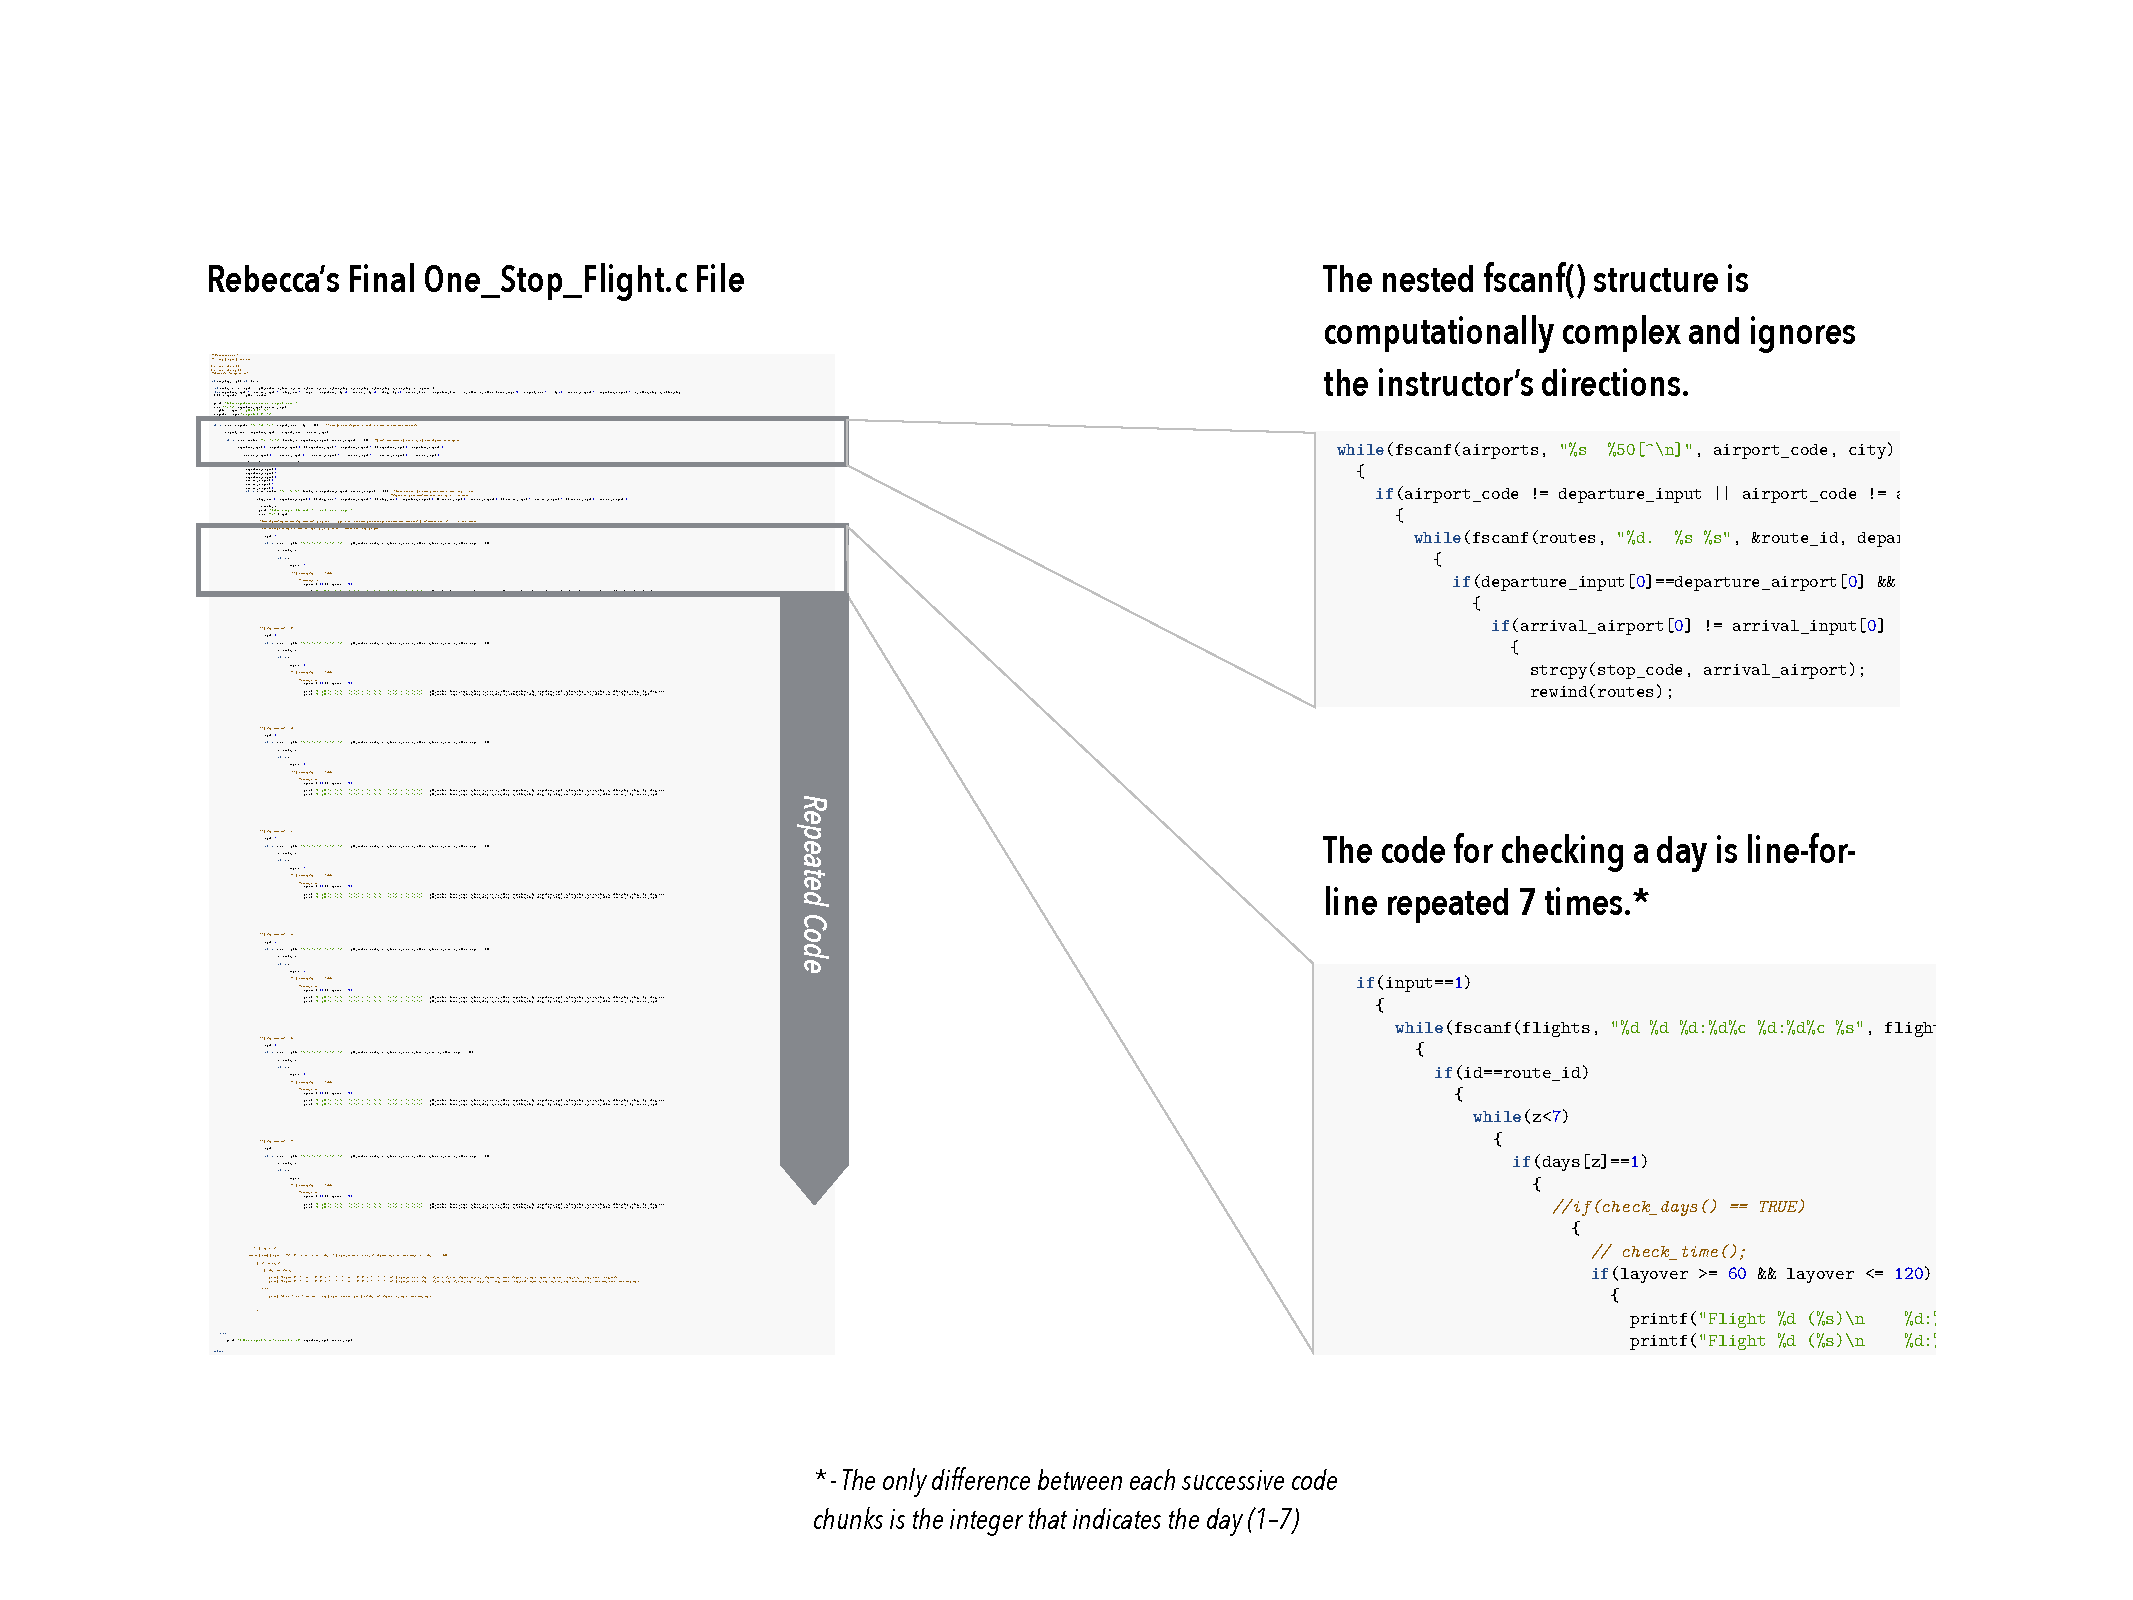
\includegraphics{RebeccasCode/OneStopFlightSupergraphic.pdf}
\caption{The entirety of Rebecca's \texttt{one\_stop\_flight.c} source code at the time her project was submitted for grading. Our final-code-only analysis focuses on two design features of this code: its multiply-nested \texttt{fscanf()} structure for handling flight data; and the seven-fold line-for-line repetition of a single block of code for checking days of the week.}
\end{figure}

\subsection{Rebecca's file-scanning solution is hard to read and has high time-complexity}\label{rebeccas-file-scanning-solution-is-hard-to-read-and-has-high-time-complexity}

After declaring variables and opening the three provided text files (flights, routes, and airports)\footnote{See Appendix A for examples of each of the three file types.}, Rebecca's one-stop flight code enters a series of conditionally-nested \texttt{fscanf()} commands. The purpose of \texttt{fscanf()} is to scan through the characters of a file, most often scanning one line at a time. The programmer can specify delimited patterns of text to look for, e.g., ``in each line, look for a word, followed by a space, followed by two digits.'' \texttt{fscanf()} also gives the programmer the flexibility to store the values of matched patterns to variables. Here's an annotated explanation of file-scanning pattern Rebecca uses on line 24 of her code:

\begin{Shaded}
\begin{Highlighting}[]
\NormalTok{fscanf(               }\CommentTok{// Read in a line of data}
  \NormalTok{routes,             }\CommentTok{// From the file called 'routes'}
  \StringTok{"%d.  %s %s"}\NormalTok{,       }\CommentTok{// Match the pattern (integer) (string) (string)}
  \NormalTok{&route_id,          }\CommentTok{// Store the value of integer to the variable route_id}
  \NormalTok{departure_airport,  }\CommentTok{// Store the value of the first string to departure_airport}
  \NormalTok{arrival_airport     }\CommentTok{// Store the value of the second string to arrival_airport}
\NormalTok{)}
\end{Highlighting}
\end{Shaded}

``Once you find a word followed by two digits, store the word in the following location in memory, and store the digits in this other location in memory.'' What's interesting isn't \emph{that} Rebecca used \texttt{fscanf()} to read through files like the list of airports. Any suitable solution for this project would need extract text patterns from source files, which \texttt{fscanf()} does. Rather, what's interesting is \emph{how} she uses \texttt{fscanf()} in her design.

Rebecca's file-scanning logic never persistently stores the contents of the files it reads in. Rather, her program reads through files one line at a time, and it essentially can't process or act on airport/flight information not in the line currently being scanned. Instead, it's been designed to copy single patterns temporarily, then rewind the file back to the top and start reading in one-line-at-a-time again.

What's consequential about Rebecca's design choice? Computationally, her code has to repeatedly open multiple files (or sometimes repeatedly open the same file multiple times) and scan lines one line at a time in order to coordinate information. So, the task of finding a one-stop flight between two cities becomes a series of repeated, one-line-at-a-time scans of external files:

\hypertarget{fscanfPattern}{\label{fscanfPattern}}
\begin{Shaded}
\begin{Highlighting}[numbers=left,,firstnumber=20,]
\KeywordTok{while}\NormalTok{(fscanf(airports, }\StringTok{"%s  %50[^}\CharTok{\textbackslash{}n}\StringTok{]"}\NormalTok{, airport_code, city) != EOF)   }\CommentTok{//scan for the departure code but not to the arrival code}
  \NormalTok{\{}
    \KeywordTok{if}\NormalTok{(airport_code != departure_input || airport_code != arrival_input)}
      \NormalTok{\{}
        \KeywordTok{while}\NormalTok{(fscanf(routes, }\StringTok{"%d.  %s %s"}\NormalTok{, &route_id, departure_airport, arrival_airport) != EOF)  }\CommentTok{//finds the name of the city of the departure airport}
          \NormalTok{\{}
            \KeywordTok{if}\NormalTok{(departure_input[}\DecValTok{0}\NormalTok{]==departure_airport[}\DecValTok{0}\NormalTok{] && departure_input[}\DecValTok{1}\NormalTok{]==departure_airport[}\DecValTok{1}\NormalTok{] && departure_input[}\DecValTok{2}\NormalTok{]==departure_airport[}\DecValTok{2}\NormalTok{])}
              \NormalTok{\{}
                \KeywordTok{if}\NormalTok{(arrival_airport[}\DecValTok{0}\NormalTok{] != arrival_input[}\DecValTok{0}\NormalTok{] || arrival_airport[}\DecValTok{1}\NormalTok{] != arrival_input[}\DecValTok{1}\NormalTok{] || arrival_airport[}\DecValTok{2}\NormalTok{] != arrival_input[}\DecValTok{2}\NormalTok{])}
                  \NormalTok{\{}
                    \NormalTok{strcpy(stop_code, arrival_airport);}
                    \NormalTok{rewind(routes);}
                    \NormalTok{departure_airport[}\DecValTok{0}\NormalTok{]=' ';}
                    \NormalTok{departure_airport[}\DecValTok{1}\NormalTok{]=' ';}
                    \NormalTok{departure_airport[}\DecValTok{2}\NormalTok{]=' ';}
                    \NormalTok{arrival_airport[}\DecValTok{0}\NormalTok{]=' ';}
                    \NormalTok{arrival_airport[}\DecValTok{1}\NormalTok{]=' ';}
                    \NormalTok{arrival_airport[}\DecValTok{2}\NormalTok{]=' ';}
                    \KeywordTok{while}\NormalTok{(fscanf(routes, }\StringTok{"%d.  %s %s"}\NormalTok{, &route_id, departure_airport, arrival_airport) != EOF)  }\CommentTok{//now searches for the place where the stop is the}
                      \NormalTok{\{                                                                                      }\CommentTok{//depart airport and the arrival input is correct}
\end{Highlighting}
\end{Shaded}

\begin{enumerate}
\def\labelenumi{\arabic{enumi}.}
\tightlist
\item
  Scan the \textbf{airports} file one line at a time (line 20)
\item
  While scanning a given line containing an airport code/city pair, scan the file of pairwise airport \textbf{routes} one line at a time (line 24).
\item
  To find possible connection cities, scan the \textbf{routes} file one line at a time again (line 38)
\item
  If a route matches, scan the \textbf{flights} file one line at a time to verify whether the time/day constraints are acceptable (one of the following lines depending on the chosen day: 52, 79, 106, 134, 162, 190, 218).
\end{enumerate}

Rebecca's code is both visually and computationally complex. The multiply-nested blocks can make it difficult for a human reader (or grader) to follow the code flow, which may have made it challenging for Rebecca to debug her own work. Moreover, nested for- and while-loops increase dimensions of complexity in Rebecca's program---what computer scientists would call the ``Big-O'' characterization of her program \citep{cormen_introduction_1990}. For every nesting of a scan loop (there are 4 in her submitted code) Rebecca increases by 1 the degree of a polynomial that represents the execution time of her program. So, from a performance perspective, Rebecca's design suffers a trade-off in that with each invocation of a scanning loop, we see a geometric increase in the time complexity of her program. But, Rebecca's code also has a particular kind of elegance.

\subsection{Rebecca's file-scanning solution has elegant constant space complexity}\label{rebeccas-file-scanning-solution-has-elegant-constant-space-complexity}

While Rebecca's design isn't optimized for speed, it uses drastically less memory than do other solutions (including the instructor's official solution). What Rebecca could have done (and what I'll discuss in a later section) is read the entire contents of all data files into RAM. I'll call that approach an \emph{in-memory} solution, because all of the flight information is loaded into memory. Instead, her solution stores only a handful of lines (4 at most) in memory at a time, leaving the rest \emph{on-disk}. An analogy helps clarify the difference.

If we think of the input files like a giant grocery list, an in-memory solution would be like having to put each list item into your cart before you go to check out. The longer the list gets, the bigger cart you'd need to collect every item on the list before checking out. Crucially, everything has to go into the cart before it can be purchased. If the grocery list very long, you may need multiple carts. If the list gets absurdly long you may even exhaust all carts in the store and still find yourself with an unfinished list.

Rebecca's \emph{on-disk} solution would be like restricting yourself to a single, small grocery basket, but taking as many trips as you need to get all the itmes from the store shelves to the checkout conveyor belt. She can only ferry just a few groceries each go-around. But no matter how long the list gets, she'll never need more than a single handbasket to get all her items to checkout. She just takes more trips.

The reason for comparing an in-memory to an on-disk solution is that design work always operates under constraints. Sometimes (say, in cloud computing applications) RAM is cheap, and a solution that loads all data into RAM may be optimal. But, there are also applied situations (biomedical implants, space technology) where memory is expensive and possibly not even upgradeable. In those contexts, a constant-space solution like Rebecca's might be ideal, because designing for the long-term means assuming a computer we launch into space now and can't ever touch again for years or decades.

But, while we know the structure of Rebecca's design, we know almost nothing about its context. Our analytical method---examining only the code in front of us---forecloses possibilities of recovering those details. We lack access to activity history: we don't know \emph{how} Rebecca ended up structuring her code this way, nor do we know \emph{why}. And, we lack access to conceptual information: we can't know from just this code whether Rebecca knew or understood the kind of complexity and performance trade-off she made. We also can't know with certainty how she felt about the consequences of the decision. We know only that her final submitted design used multiply-nested scanning loops.

\subsection{Rebecca's file-scanning solution ignores an assignment directive}\label{rebeccas-file-scanning-solution-ignores-an-assignment-directive}

For each of the four projects during the semester, the instructor gave students what he called a ``design brief.'' Each design brief outlined the problem to be solved as well as any constraints imposed on students' solutions. For example, in the flights project, students' programs had to reject candidate multi-stop trip routes if the layover time would be too short (under 30 minutes) or too long (more than two hours). But, in addition to what I might call \emph{user-centered constraints} (viz., reject multi-stop trips that would have grueling layovers), the instructor also directed students on \emph{implementation details}: ways their program should work at a technical level that would be invisible to the user.

Specifically, the design brief discusses how to handle reading in data from the files provided for the project:

\begin{quote}
To parse the 3 airline flight database files, you will need to declare arrays that will receive all the data. For the purposes of determining array sizes, you may assume there will never be more than 100 airports in the ``airports.txt'' file, 500 route IDs in the ``routes.txt'' file, and 3000 flights in the ``flights.txt'' file. (Flights Database class assignment, 2012)
\end{quote}

Presumably, from the instructor's directive, one ``will need'' to have an array of airports (mapping 3-letter code to full airport name), an array of routes (mapping a pair of airports to a unique routing number), and an array of flights (mapping unique flight numbers to a collection of information about that flight). And, to fulfill that need as stated, a student's code would have to:

\begin{itemize}
\tightlist
\item
  Create arrays by declaring them as variables
\item
  Store data from the files in array entries using variable assignment
\item
  Access the arrays to fetch relevant flight data
\end{itemize}

Rebecca creates no arrays. Instead, her code attempts to accomplish the same task that an array would, but she doesn't use a global data structure at all.\footnote{That's not entirely true. Technically, variables including \texttt{route\_id} and \texttt{flight\_number} are globally-acessible within the scope of the \texttt{one\_stop\_flight()} function. But, those variables are integers. There's no way the variables Rebecca declares could store all the data required in-memory.} A consequence of Rebecca's approach is that she has no easy way to refer to arbitrary airports, routes, or flights in her code, since her program has no mechanism to store such information persistently. A second consequence is that since she avoids persistent data structures, the complex work her program does to read through each line of each file, in some cases multiple times (above) is repeated every single time a user initiates a query.

Given Rebecca's particular design pattern, we asked the question of whether she may have tried creating arrays before ultimately settling on her scanning-loop solution. The answer, as far as we can tell, is no. We analyzed the history of both Rebecca's main() method and her one-stop flight code module. Our search revealed that no snapshots exist in which Rebecca created arrays---either through dynamically allocating them (through heap memory), or, as the assignment recommended, creating overprovisioned fixed-size arrays on the stack. In other words, at the limit of resolution of our data collection, and within the scope of the code Rebecca typed, she never tried an array solution.\footnote{If Rebecca had tried an array solution and compiled---whether error-free or not---our automated snapshot collection system would have captured it.}

Curiously, we have evidence \emph{outside} of Rebecca's code that suggests she knew, and even perhaps had seen, an array-based design solution. In a file called ``notes.txt'' contained in her project directory, we see the following lines:

\begin{verbatim}
think about using: sscanf, array of pointers


his header file!!!
-max line lenght: 2000
-max string lenght: 100
-defined true and false
-max airports: 100
-max routes: 500
-max flights: 3000
-min connect time: 60.0
-max connect time: 120
-daily maxk: 254  ???
-char airports[max airports][4]
-char aiport_cities[max airports][max string lenght]
-he has 3D array for routes.... char routes[max routes][2][4]
\end{verbatim}

(notes.txt file, created March 19, 2012)

The context of the file is not entirely apparent, because we did not observe lecture on March 19, the day the notes.txt file entered Rebecca's snapshot history. Also, whether ``his'' refers to the instructor or perhaps another classmate is unclear. ---What seems clear, however, is that Rebecca was responding to items she had seen in someone else's header file. Consequently, putting together the notes.txt file with Rebecca's final code submission reveals Rebecca was exposed to a design solution involving arrays, but never implemented it in her code. Thus, a lingering and consequential question remains unanswered: why did Rebecca adopt a solution that defied the directions of the assignment, especially when she'd seen part of a potential design solution that did use arrays?

We return to this question in a later section, but first we turn our attention to another unusual feature of Rebecca's work: seven-fold repetition of code.

\subsection{Rebecca repeats the same chunk of code seven times}\label{rebecca-repeats-the-same-chunk-of-code-seven-times}

A second key feature of Rebecca's code is the almost identical repetition of a single 23-line code chunk seven times (lines 50--240). Because users can run queries by choosing a day to fly (and some flights only run on certain days), students' code must be able to handle each of the seven possible days for when a user would want to fly. In principle, Rebecca's code achieves just that.\footnote{I say ``in principle'' because Rebecca's code would not compile on my machine. So, in practice, her design contains compile-time errors (and possibly run-time errors). Nevertheless, her code provides ample evidence that she was attempting conditional logic to handle each possible day.} In practice, her code creates seven different conditional branches---one branch for each day of the week---where the code within each branch is duplicated.

Figure 2-1 represents a side-by-side delta-comparison of two such day-specific branches of code. Lines 158--184 of Rebecca's original code are on the left; lines 214--241 are on 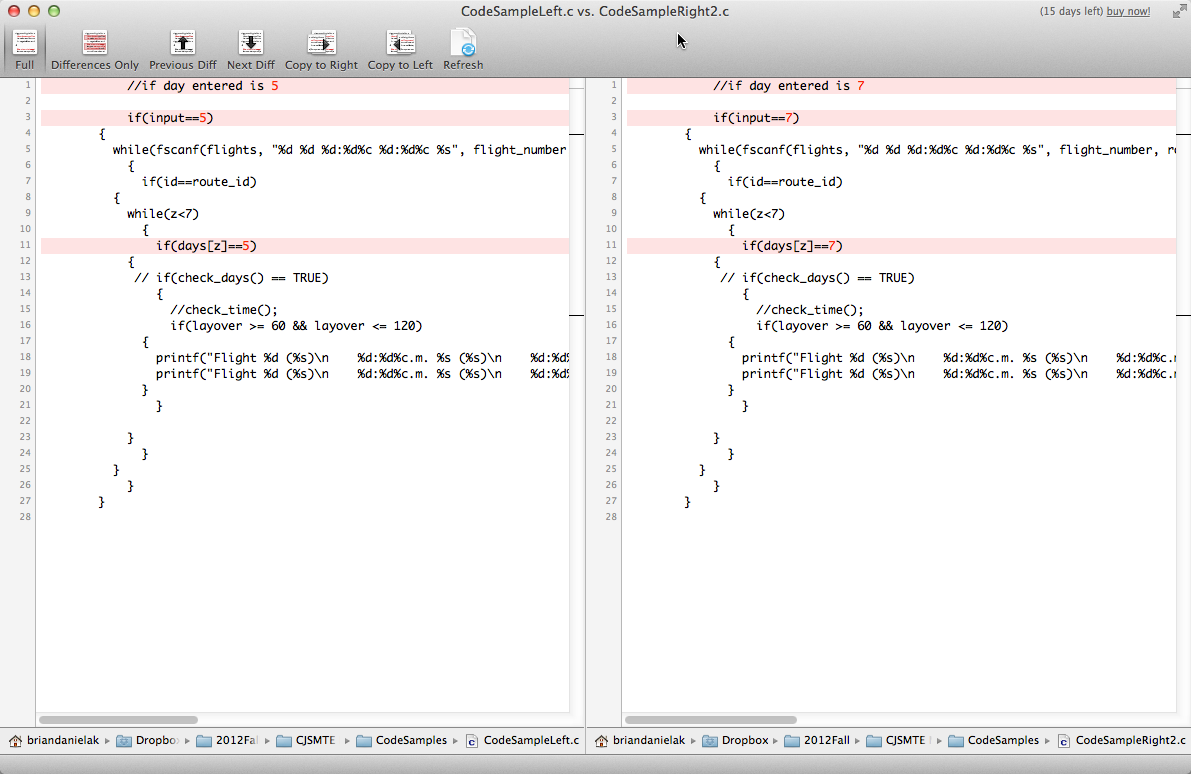
\includegraphics{media/media/image3.png}the right, and in the figure lines have been renumbered (from 1) to ease comparison. In this delta view, lines that differ are highlighted in pale red, and characters that differ are shown in bold red.

The two code blocks demonstrate just how much code is duplicated for handling user input based on days of the week. Between these two chunks there are only three differences (lines 1, 3, and 11): all of the references to day are changed from 5 (on the left) to 7 (on the right).\footnote{In the text-input files students were given, days of the week were represented as integers (rather than the perhaps more familiar ``Tuesday,'' ``Wednesday,'' etc.).} Moreover, the changes from block to block are patternistic and predictable: the first line of the block is a non-functioning comment, the third line of each block just checks whether the rest of the block should run, while the eleventh line of each block compares an array entry to the day of interest. Everything else is duplicate boilerplate that is essentially repeated 7 times; once for each day of the week. I say ``essentially repeated'' because, as we'll now explore, there are minute differences between some of the code chunk's seven incarnations.

Repeating code as Rebecca has done can be problematic because each repetition multiplies the number of places she has to examine and modify if she wants to introduce a systematic change. If, for example, Rebecca wanted to change the internal names she gives to scanned-in variables, she has to make that change in seven different blocks of code: once for each of the seven days of the week she's hard-coded. And, since any given change may inadvertently introduce an error, increasing the number of places she repeats code also makes the code that much more vulnerable to inconsistently-applied changes.

Indeed, a repeated, inconsistently-applied scan pattern change seems to be exactly what occurred in Rebecca's code history. Between 10:04pm and 10:37pm on March 26, Rebecca introduced a large set of changes to the one-stop flight module. Among those changes Rebecca added the \texttt{d\textbackslash{}\_letter} file-scanning-parameter to what would become line 218, but not to what would become line 190. We can reasonably infer Rebecca added this parameter as a way of capturing the ``am'' or ``pm'' specifier given the input file's format. Moreover, we can verify through Git that once introduced, Rebecca's omission of the parameter was never modified or corrected. The problem percolated through to her final submitted code.

\section{Analysis Augmenting Code Snapshots with Interview Data}\label{analysis-augmenting-code-snapshots-with-interview-data}

In the previous section, I described two unusual features of Rebecca's code for searching one-stop flights:

\begin{enumerate}
\def\labelenumi{\arabic{enumi}.}
\item
  Her use of multiply nested loops that scan through source information files \emph{without} storing the information in those files persistently in long-term memory

  The code for handling a user's chosen day, which was essentially the same block of code copied and pasted 7 times
\end{enumerate}

In this section, I offer explanations of Rebecca's design choices by interpreting data from over five hours of clinical interviews I conducted with her. I draw from those interviews to explain how design decisions that might seem unusual to an expert in fact grew rather unproblematically (for Rebecca) as ways of deliberately transferring prior knowledge and designs (which explains feature 1) or coping with a constraint to produce a reliable solution she could trust (which explains feature 2).

\subsubsection{Rebecca employed fscanf loops because she was deliberately reusing from an Basic Programming Assignment.}\label{rebecca-employed-fscanf-loops-because-she-was-deliberately-reusing-from-an-basic-programming-assignment.}

Rebecca's choices become easier to understand when you consider what she said in the interview. When Rebecca initially saw the flights database project, her first reaction was ``this is just a lot like our fantasy football project that we did last year'' (Interview, March 16, 2012).\footnote{Transcript conventions are shown in Appendix 1.} But, the previous fantasy football project was easier because all of the information she needed was in one file. Flights database, by comparison, fractured necessary information across multiple input files.

Since Rebecca said the fantasy football project was like an easier version of flights database, I asked whether she tried making this project more like the easier one. Her response was an emphatic ``Oh yeah! Definitely!'' (Interview, March 16, 2012). She said ``as soon as we got this project I was like, ah! fantasy football! I'm just gonna go and see how much code I can rework from that and like, use /mmhmm/ in this project'' (Interview, March 16, 2012). Specifically, Rebecca went back to her fantasy football code ``and I was looking at how I scanned in the information from the files, cuz, we haven't really done anything like that this semester. Uh, scanning in from files before---'' (Interview, March 16, 2012). Since the fantasy football draft project was the last in which she'd needed to do file-scanning, she ``just, uh, went back to check how I did that /mmhmm/ and then, if I could I copied, but because a lot of the variables were different, uh, like these were more var---less, less variables, and more strings than last year /mmhmm/ uh, I just retyped it out. I just looked at how it was similar'' (Interview, March 16, 2012).

My first opportunity to discuss Rebecca's one-stop flight work was on March 16, 2012, in what would be her third of five interviews that semester. This interview was conducted very early into the time window for the Flight Database project, before Rebecca had done the bulk of her coding. We were discussing her prospective design plans. As Rebecca began explaining how the logic for a one-stop flight search was supposed to work, she described what she saw as one of the central difficulties of the project: the relevant information for answering user queries was spread across multiple files (Interview, March 16, 2012).

As Rebecca explained, something as simple as finding a flight from, say, JFK to BWI ``involves scanning through multiple files, because it's not like one file that has everything conveniently like, there'' (Interview, March 16, 2012). When I asked what would make things easier if, hypothetically, all the information she needed were in one file, Rebecca responded by appealing to a previous assignment from last semester. In Rebecca's first-semester programming course (Basic Programming for Engineers), one of several multi-week projects had students create a system for users to conduct a fantasy football draft. The project involved, among other things, topics related to basic file management in the C language, including how to read in a file from disk (Interview, March 16, 2012). Rebecca explained:

Rebecca: Um, like, cuz when we first got this project, uh, I actually was thinking ``oh, well this is just a lot like our fantasy football project we did last year.'' /Huh/ We uh, had to scan in, uh, someone had to enter like ``I wanna pick a quarterback,'' so then you had to scan in and go and look for all the quarterbacks in the file and say ``OK, this is the quarterback'' and everything. But, in that project we only had the one file that had everyone listed: quarterbacks, runningbacks, wide receiver, in one file. And all the information you needed there /Mmhmm/ So, you could just get it all and compare it all at once with one scanf /mmm/ whereas this you have to, take, uh, you scan in the flights, ah, the flights file. So, then you find the flight number. You have to save the ID from that flight number, use that ID to scan into the routes file /mmhmm/ and then save the routes information and then print it out with the flights information. (Interview, March 16, 2012)

Rebecca's comments suggest she saw a coupling between the arrangement of the input information and the structure (and complexity) of the computational logic needed to process it. When one fantasy football file contained all of the relevant information (player, position, team, etc.) it could be read in and processed one line at a time. When information was fractured across files (pairs of airport codes in one file, full spell-outs of airport names in another, for example), Rebecca felt she'd need to use information shared across files (such as a route ID) to coordinate a scan across one file with a scan across another (and possibly an additional scan across a third file) before she would have all the necessary information and computations to return a result.

I was interested in the connections Rebecca saw across projects, so I pressed on. When I asked whether she thought about trying to make this project like her fantasy football project, her answer was an emphatic ``Oh yeah, definitely!'' As she elaborated:

Rebecca: That was like, as soon as we got this project I was like, ah! fantasy football! I'm just gonna go and see how much code I can rework from that and like, use /mmhmm/ in this project. And, my whole main file, like all those NULL checks and everything, I mean they're really simple to write, but I just copied `em and put `em there, cuz, we had the same thing. /Mmhmm/ Um, just changed, like, the names of the files.

As she explained, ``reading in files'' was a topic covered extensively in Basic Programming---the first course of the sequence---but they hadn't talked much about it in this semester's course.

Rebecca: Because \[reading in from files\] was a big \[Basic Programming\] topic we hadn't talked about it much. /Yup/ So, I just, uh, went back to check how I did that /mmhmm/ and then, if I could I copied, but because a lot of the variables were different, uh, like these were more var---less, less variables, and more strings than last year /mmhmm/ uh, I just retyped it out. I just looked at how it was similar. (Interview, March 16, 2012)

I started doing the scanning, and then I realized like, ``I do not have all the information I need in this one file,'' so that's when I realized I would have to make the dummy variable to compare to the other file, so, which, there was no other file in the, um, fantasy football one. So that's when I realized, I was like OK, so, there's gonna be other stuff that I'm gonna have to do, and /mmhmm/ I mean, I can still kinda compare cuz it's still scanning files /yup/, but the idea of the dummy variable and all that, that would not have come from fantasy football, so /sure/.

In sum, then, Rebecca's repeated, nested scan loops were a structure she deliberately borrowed from a previous semester's project. By her telling, what seemed obvious was that ``scanning in from files'' was a topic she'd already covered, which meant she'd already developed a workable solution for how to solve that problem. Thus, she saw the problem of how to coordinate airport information from different files as a new instance of the old problem of reading information in from one file. Her flight database work, accordingly, tried opportunistically adapting a previously working solution to fit the current circumstances.

\subsubsection{Rebecca repeated code because she wanted to re-use functionality she could trust}\label{rebecca-repeated-code-because-she-wanted-to-re-use-functionality-she-could-trust}

By our interview on April 6, Rebecca had already completed and submitted her code for the flights database project. When I looked at the final form of her code for finding one-stop flights I noted an unusual pattern described in section 2.4.3 above: she had a code chunk repeated almost character-for-character 7 times. In the interview, this section is what Rebecca referred to as ``my obnoxiously long part of my code'' (Interview, April 6, 2012):

Rebecca: So, the way I did it was really long and probably, there was probably like a much easier way, but I just did a giant if---if statements \{swings cursor from line 50 to line 63\} If they wanted to fly on Monday /OK/ I went through and checked to see if the route ID was the same \{wiggles cursor across line 54\}, and if it did, I went through to che---uh, I made a check\_days function \{wiggles cursor across line 60\} uh, I ended up commenting that out cuz I didn't end up /mmhmm/ finishing it. But, uh, my check\_days function worked, it just didn't work completely with the code /OK/ (Interview, April 6, 2012)

As I scrolled the screen to look at each of the repeated blocks of code, Rebecca elaborated:

Rebecca: And this is why my code, I feel like, is not uh, concise enough, or, I don't really, I forget the word they use, but uh /\{inaudible\}/ it's very long because I couldn't figure out if I should do a while loop or whatever /Uh-huh/ But, so I was just like, I know this way should work if I get everything else right, that uh, just go through, if input's 1, if input's 2 and just do the same thing in each of `em just /Mmmhmm/ check for, ``oh, if days is 2, if days is 1'' instead of, like---Cuz I probably could have done, like, maybe a giant while loop, um, to try and, and if, while, inputs something, uh, then you check to see whatever i is. But, I could, I didn't---couldn't figure out how that would work, so I just did the same thing six times.

Interviewer: So, in, in each one of these it's like, looks, and I'm not sure about this, but it looks like the way you wrote it---so this \{highlights line 79\} is pretty much the same in all of them, right? /Yes/

Interviewer: So's this one \{highlights line 81\} /Yes/ this one \{highlights line 83\} Here's where it's different \{highlights line 85\}

Rebecca: Yes, because it just checks if it's a 2 instead of a 1.

Interviewer: OK. Um. /And then everything else is still the same/ Layover's still the same. OK.

Rebecca: Yeah. So that's why it's prob---it's not, uh, the neatest code or whatever, because it's the same thing six times. (Interview, April 6, 2012)

Given Rebecca's assertions that her code wasn't neat, I asked what, if anything she might change if she hypothetically had another week to work on the project.

Rebecca: Um, first I'd try and get it to make sure it worked completely /Ahh, OK, yeah/ this way, \{laughs\}, uh, and then, if I had the week after that whatever, I'd probably go through and see if I could figure out a way to make it concise-r because he likes uh, neat, as, like, code that's, uh, easy for the user to see /uh-huh/ I guess. Uh, I forget what, I keep forgetting what the word he used was at the beginning of the year, but uh, just very concise and, uh, this is \[a\] very expanded \{laughs\} way of coding, but, it made sense to me at the time and I was just like ``I just want something that makes sense right now.'' /Right/ So, that I can actually work with and have an idea.

Interviewer: Um, OK. So, so it would take you some extra thinking to figure out /Mmmhmm/ how to break this down into /Yes/ smaller stuff /smaller code/ Do you feel like you've had a lot of practice doing that, or like?

Rebecca: Uh, a little. Like, but, a lot of times in \[Basic Programming\] they didn't really mention too much about being concise. They were just like ``if you can do it, do it'' \{laughs\} /OK/ So I usually stuck to what made sense to me /Right/ uh, to turn the projects in. (Interview, April 6, 2012)

In summary, Rebecca's ``expanded way of coding'' was a way of expressing ideas in code that, in her own words, ``made sense'' to her. Moreover, her Basic Programming course seemed, to her, to set expectations that functionality comes first; ``neatness'' second. If she hypothetically had more time to work on the project, her first priority would be to get her existing code working. Consequently, Rebecca's repetition of code can be understood as a kind of pragmatic solution to a difficult problem: choosing which computational techniques were best for accomplishing a complex goal. Moreover, her approach was shaped by the fact that her Basic Programming course historically valued a philosophy of ``if you can do it, do it'' (Interview, April 6, 2012). Ultimately, those factors seem to be what led Rebecca to choose repeating code that made sense to her over the difficult-to-envision alternative of a ``giant while loop.''

\section{Discussion}\label{discussion}

When we consider evidence from both code snapshot histories and clinical interviews with Rebecca, we can draw several plausible conclusions about Rebecca's patterns of software development on this project. Moreover, those conclusions can spur larger considerations about theorizing student learning and considering alternative instructional strategies that may be more responsive to student needs. Below, I synthesize and discuss patterns in Rebecca's development.

\subsection{Rebecca's key design decisions are made early, persist through to her final submission, and carry consequences}\label{rebeccas-key-design-decisions-are-made-early-persist-through-to-her-final-submission-and-carry-consequences}

On both her non-stop flight code and her one-stop flight code, key structural features of how Rebecca's code works never meaningfully change after Rebecca introduces them. In particular, Rebecca's use of fscanf() patterns (as opposed to storing the data persistently in memory) occurs extremely early in the work history of the project. The fscanf() patterns initially appear in Rebecca's flight-checking code on March 19, the third of what would be 286 chronological snapshots we have comprising Rebecca's work on the project.\footnote{The project was distributed to students on March 5 and was due March 28, but the bulk of Rebecca's work on the project (284 of the 286 snapshots) occurs beginning March 19. \url{https://github.com/TLPLEngineeringEdResearch/Rebecca/compare/e0a7caab4eb2d8401a0e50e8c6c6d8b514e9054e}\ldots{}0e8a5c606ef30f3b404024fdfad17d8d50e32456} We note several consequences that arise \emph{because} these design choices were made early and persisted to the final code.

First, Rebecca's \emph{early} choice not to persistently store data likely forced her into the complicated scanning loop logic she developed \emph{later} to solve the one-stop flight problem. A bit of explanation may help here. Because the database students were building has multiple uses, including uses that find flights for users, to be successful Rebecca had to write functionality that found both non-stop and one-stop flights for users. But, Rebecca initially designed each part of her code---airport listings, flight listing, non-stop flight search, and one-stop flight search---with its own internal fscanf() loops, as opposed to having the four of them each refer out to a separate module that could handle reading in data. The result is that none of her individual modules share file-scanning code, and repeat data look-ups necessarily have to be handled by creating another nested scan loop. A design where code with a common function is pasted repeatedly into separate modules contrasts strongly with one in which separate modules all refer out to a single external piece of code.\footnote{As an analogy, imagine a supermarket where every unique type of item on the shelf has a cash register specific to that item next to it. To buy an item shoppers have to check-out individual items as they move through the store. It's a pain for shoppers because shoppers have to swipe their cards at dozens of separate item-specific registers across the store just to pay for a single grocery run. It's a pain for store-owners because now there are literally hundreds of individual registers to manage, maintain, and upgrade.}

We can understand Rebecca's development as involving a kind of design inertia. Because she decided from the start to scan information using fscanf() separately in each module, her later code was also beholden to that commitment. The end result is that increasing the problem complexity a small amount (the challenge of handling one-stop flights versus non-stop flights) forces her to write much more code that is itself more complex in its flow of control. And, when we consider her seven-fold repeated code for checking flight availability on given days, there are similar consequences. The decision---whether intentional or not---to create seven different conditional paths forces Rebecca to write and maintain much more code over time as the project evolves. As we suggested in section 2.4.3, having a large number of locations to keep in sync is likely what made Rebecca vulnerable to one of the errors she ultimately introduced into her code.

\subsection{Her design decisions may be influenced by framing and overzealous transfer}\label{her-design-decisions-may-be-influenced-by-framing-and-overzealous-transfer}

Rebecca said in our interviews that she explicitly tried to reuse solutions from the previous semester's fantasy football project. Our code snapshots help us understand the extent to which that's true. Rebecca's first compile for her flights database work begins with this commented line of code:

//Rebecca Wells's Fantasy Football Team Maker: Project 1

Thus, our interview with Rebecca corroborates the snapshot evidence that Rebecca directly copied code from a prior project. Moreover, Rebecca's behavior of copying her old fantasy football code suggests several implications.

First, to extend our point in section 2.6.1, Rebecca's ``design inertia'' actually traces as far back as the decisions she made during the first project of her first semester of programming. That is, by copying code (and particularly file-scanning logic) from an old project, she was incorporating core functionality that she designed when she first learned to program. Admittedly, code reuse isn't in and of itself a problem in software development. Parson and Saunders (2004), for example, have written on cognitive heuristics that keep professional software engineers from reusing code, even when reusing and extending existing software artifacts is the best course of action on a software project. So, the concern isn't that Rebecca reused code, but rather the matter of what cognitive dynamics were at play that directed her choice to reuse that code. In that regard, the constructs of framing and transfer may help us better understand Rebecca's activity.

Framing, as it has been applied in contexts such as physics education (Elby \& Hammer, 2010; Hammer et al., 2005; Scherr \& Hammer, 2009) and mathematics education (van de Sande \& Greeno, 2012) concerns how participants understand the social and intellectual activities in which they're engaged. Of particular relevance to studying Rebecca is the notion of \emph{epistemological framing}, which van de Sande and Greeno (2012) summarize as

participants' understanding of kinds of knowledge that are relevant for use in their activity and the kinds of knowledge, understanding, and information they need to construct to succeed in their activity (e.g., what kind of information would count as a solution to the problem they are working on). (van de Sande \& Greeno, 2012, p.~2)

Rebecca's decision to copy code from fantasy football implicitly reflects her orientation toward what kinds of knowledge (the course topic of scanning information from files) are relevant to solving the problem. More broadly, note that in Rebecca's interview she explains that her primary objective is to get a solution that works, which stands in contrast to having a design priority like having a solution that is elegant, or one that transparently manages complexity. That commitment again reflects a manifestation of epistemological framing as ``what would count as a solution,'' where for Rebecca what counts is a solution that works.

Additionally, Rebecca saw the flight database project as a new instance of a prior problem: fantasy football. Consequently, she consciously adapted past solution patterns, because the flights database project looked like it contained problems she had already solved in previous code. Rebecca's deliberate reuse of old code can be readily understood as an example of what Schwartz, Chase, and Bransford (2012) call ``overzealous transfer'':

Of particular concern are situations where students transfer skills, knowledge, and routines that are effective for the task at hand but may nevertheless be sub-optimal in the long run because they block additional learning. We will call this \emph{overzealous transfer} (OZT)---people transfer solutions that appear to be positive because they are working well enough, but they are nevertheless negative with respect to learning what is new. (Schwartz et al., 2012, p.~206)

In short, when students overzealously transfer prior knowledge as Rebecca did, ``they may believe they are doing the right thing, and without appropriate feedback they cannot know otherwise'' (Schwartz et al., 2012, p.~206).

In Rebecca's case, the constructs of framing and overzealous transfer together let us describe why she would have repurposed a solution that she felt was adequate, even to the exclusion of the topics being taught in class and the explicit directions in the project brief. By framing the flights database problem as a new instance of an old problem, Rebecca treated it as she did the old problem. But, she arguably transferred \emph{too} \emph{much} of the old code's structure; so much that she had to introduce even more complexity into her code just to make the transferred parts work properly under the new constraints. And, because her framing of the task seemed to privilege a philosophy of ``if you can do it, do it'' (Interview, April 6, 2012), her primary goals were to get her program to work, by whatever means she could understand and trust.

\subsection{Conclusion}\label{conclusion}

In closing, even with a complete snapshot history and over five hours of clinical interviews, it's still an enormous challenge to thoroughly understand one student's design trajectory on a project. The challenge is both methodological and theoretical. Through interviews we know what Rebecca was thinking retrospectively, but we still work at a remove from understanding what she was thinking in the precise moments she wrote her code. Conversely, our snapshots provide a detailed record of the state of her code every time she compiled. But, our snapshots are limited by the kinds of materials they can track and the frequency with which they're taken. We don't know, for instance, what Rebecca might have been talking to others about while sitting in a dorm lounge working on her project. And, because Rebecca wouldn't always compile frequently, some snapshots detail large changes to the code made over long periods of time---hours or days---which can limit our ability to precisely determine what happened, and when.

From a theoretical perspective, we find our attempts to understand her design decisions involve appeals to constructs of a finer granularity and dynamism than are typically considered when studying first-year programming courses. Understanding why fscanf() loops dominate Rebecca's flight search code, for example, pushes us to consider the effects of how Rebecca framed the task and the subsequent overzealous transfer that resulted. And, understanding why code gets repeated seven times pushes us to consider how emotion couples with sense-making in students' design decisions. In Rebecca's case, a time-pressured preference for code that ``makes sense right now'' translated to a design of explicitly repeating procedures instead of elegantly abstracting them.

\section{Conclusion}\label{conclusion-1}

If there is one overarching finding from this dissertation, it's that students clearly have resources for thinking about designing programs and a diversity of approaches to programming in the moment. Below, I explain the kind of diversity I saw in programming approaches. Then, I conclude with a discussion of what my research might mean for assessment.

\subsection{We should think carefully about what students' programming design knowledge means for assessment}\label{we-should-think-carefully-about-what-students-programming-design-knowledge-means-for-assessment}

My research helps us document and model the kinds of knowledge students have. In so doing, it points out kinds of information that the course's assessments were apt to miss:

\begin{enumerate}
\def\labelenumi{\arabic{enumi}.}
\item
  How students frame or otherwise approach the task of programming in the moment
\item
  The role of different kinds of prior experience in stabilizing (or potentially destabilizing) certain kinds of frames
\item
  In-the-moment practices---including talking out solutions, sketching out debugging strategies, and writing out pseudo-code---that display students' competence and sense-making
\item
  The code history that traces how designs evolve, including how students start projects and what parts of their designs become dead-ends
\end{enumerate}

Together, those four points are relevant for formative assessment (Black \& Wiliam, 1998) in introductory programming. (1) and (2) point us toward what students think they're doing when they're programming. Analogous work from science education tells us that students' sense of the kind of knowledge activity they're enacting matters for learning and assessment (Russ, Coffey, Hammer, \& Hutchison, 2008). For example, knowing early on that students are blindly copying code or randomly trying syntax gives instructors a chance to intervene. But, my research suggests intervention can't just be about stopping a bad behavior: knowing that copy-paste behavior is happening is different from knowing \emph{why} it's happening.

Formative assessment has to be about diagnosing causes, not just identifying symptoms. Otherwise, we run the risk of ignoring or even harming students' productive knowledge. Take the example of copy-paste behavior, as documented by Gaspar and Langevin (Gaspar \& Langevin, 2007). One reason we may see copy-paste behavior, as Study 1 demonstrates, is that students might see situations as new instances of already-solved problems. In professional practice, seeing old solved problems in new situations can be productive. Such insights can, for example, direct engineers to use a pre-built library of functions instead of building their own. But, another related reason for copy-paste may be efficiency. For Rebecca, copying and pasting code was very fast; it required only a few quick keystrokes. In the short run, Rebecca's choice to copy the code was a faster, less demanding, more trustworthy route to go on than was abstracting the code to a function. When we consider students trying to see common problems in new scenarios and solve such problems efficiently, ``copy-paste'' becomes a symptom rather than a root cause. Epistemological frameworks, then, can inform assessments by offering explanations that aim at the root cause of certain behaviors.

Points 3 and 4 complement knowledge analysis by drawing focus to artifacts, practices, and history. As data from Lionel shows (Study 2), a crucial part of his design process involves artifacts and activities that were only distally knowable to the assessments he got in class. Lionel's instructor had no direct access to:

\begin{itemize}
\item
  Lionel's whiteboard
\item
  the hours Lionel may have spent working out designs in chalk
\item
  how Lionel might have talked out design features
\item
  how Lionel's initial ``pseudo-code'' evolved into his final design.
\end{itemize}

In Rebecca's case, commented-out code in her final project submission were perhaps the only clues at all that she tried abstracting some flight day-checking procedures into functions (Study 1). Without Rebecca's history, the instructor would have had no reliable way of knowing:

\begin{itemize}
\item
  Rebecca began her flights database project by copying code from an earlier project
\item
  Rebecca's original solution for day-checking evolved from a seven-fold conditional structure, one for each day
\item
  Rebecca may have tried abstracting day-checking procedures, even creating a function called check\_days.
\end{itemize}

To sum up: traditional assessments can tell us what students finally produce but not how they produce it, when they produce it, why they produce it, or what the production process was. In the summative assessment structure of the course, final student products were the only products submitted to the instructor. My research shows that what's happening in the interstices---before typing, between compiles, away from the computer---can be captured and, in principle, analyzed and acted upon by instructors.

\subsection{What We Might Change About Classroom Practice}\label{what-we-might-change-about-classroom-practice}

What follows is my speculation about how we might specifically change classroom practices in light of my research findings. I move from recommendations I think are most strongly supported by my data to recommendations that align with my findings but are more expansive, and thus less strongly supported. As my recommendations broaden, I try to offer not only an instructional recommendation but a concomitant question for research.

\subsubsection{Instructors could look beyond content to understand student difficulties}\label{instructors-could-look-beyond-content-to-understand-student-difficulties}

I think first and foremost, instructors have to have a willingness to recognize that the difficulties they think they're seeing in students are difficulties they may be viewing through a lens of content. For example, after seeing a student struggle an instructor might say ``the student doesn't know assignment statements.'' But, those difficulties almost certainly have a deeper explanation. I say ``almost certainly,'' where what I mean is that there are a number of patterns we've identified as common novice errors, but most research stops before asking why that's a common novice error. With rare exceptions (Fleury, 1991, 2000), the computing education community doesn't encourage asking the question \emph{why might a student be doing this?} and \emph{what might this tell me about the way a student is making sense of this?} By contrast, my research suggests those orientations are ripe, low-hanging fruit for instructors to take on. I think one of the first things as instructor could ask is, \emph{why would a student be thinking that this is the appropriate thing to be doing?} And that holds true whether the thing in question is writing the statement this way, or interpreting the code this way, or enacting this kind of programming activity this way.

Moreover, we know from research on metacognition (Schoenfeld, 1987, 1992) that thinking beyond content opens the palette of kinds of interventions an instructor can make. Schoenfeld (1987), for example, came to encourage metacognition in his classroom by doggedly asking student groups what they were doing, why they were doing it, and how they hoped it would lead them to a solution. Students ultimately came to internalize such strategies and spent far less time floundering along solution paths that weren't ultimately productive. Might the same idea be true in introductory programming courses? To find out, we could begin researching in earnest how often and in what ways instructors model metacognition for their students. Currently, I would argue, we don't know whether and how instructors do so.

\subsubsection{Instructors could use code history to inform interventions}\label{instructors-could-use-code-history-to-inform-interventions}

When, for example, a student comes to office hours with a problem on a project, an instructor needs to quickly come to grips with the state of the students' project, the logic of their design, where they're stuck, why they're stuck, and what might best help them. That's no small task. But, given my analysis I have strong reason to believe that having code history available to instructor could change both the nature of coming to terms with a student's project and the conversation with a student that results. If an instructor can see the evolution of a student's code, at the very least they could see where the student started, how the code was growing, and where the student was working most recently. Even if the instructor had never before seen the code (or its history) until that moment in office hours, having both available changes the kind of view the instructor can get of the code and the specifics of the intervention that might result. In Rebecca's case, for example, it might have been an opportunity to explore why her check\_days abstracted function was failing on her flights database project.

Having code-snapshot capabilities also changes the kind of research we can do. First and foremost, a result of this dissertation was to create a freely-available, lightweight, open-source framework for capturing and visualizing students' code histories.\footnote{\url{https://github.com/briandk/gitvisualizations}} So, the most basic kind of study would involve deploying that framework from the instructional side of a course and exploring what happens, as, for example, Hurd (2013) has done. One could ask questions of how instructors build code snapshotting into their course, how such information could or did inform assessment, and how such information could or did change the nature of instructional interactions with students. Was it for the better? If so, how do we know? If not, how do we know?

\subsubsection{Instructors could establish a norm of asking why a design choice makes sense}\label{instructors-could-establish-a-norm-of-asking-why-a-design-choice-makes-sense}

The most far-reaching implication of the research I present here is that instructors should establish a norm in their classes where anyone, at any point, for any piece of code, is allowed to ask \emph{why does this make sense as a design choice? Why is that an obvious choice to make? How does that work?} Consider a parallel example from mathematics education. In Don Saari's calculus class at UC Irvine, he ``invokes the principle of what he calls ``WGAD''---``Who gives a damn?'' (Bain, 2004, pp.~38--39). Bain explains:

At the beginning of his courses, he tells his students that they are free to ask him the question on any day during the course, at any moment in class. He will stop and explain to his students why the material under consideration at that moment---however abstruse and minuscule a piece of the big picture it may be---is important, and how it relates to the larger questions and issues of the course. (Bain, 2004, p.~39)

What I'm suggesting is even broader than that, because it's not just a question students can ask of professors; it's a question \emph{anyone} can ask of \emph{anyone.} I see it as the programming and design extension of a sociomathematical norm (Yackel \& Cobb, 1996), and I think it could lead to collaborative sense-making. That is, I'm asking for an accepted cultural practice that is also itself a design practice, whereby an instructor can help create a safe, stable space for a community to be reflective and critical about design choices. I also think it's an idea that leads to others, such as letting, if not requiring, students review one another's code. When students are forced to reckon with someone else's code and understand their design decisions, they're also forced to justify their own decisions. And establishing ``why that design choice?'' or ``how does that make sense?'' as a norm provides reciprocal opportunities for students, not just instructors, to improve the code of others.

The research questions that come out of such an idea would include:

\begin{itemize}
\item
  How can an instructor satisfactorily establish norms about design in a classroom?
\item
  What does it look like when students collaboratively sense-make about a program's design choices?
\item
  What does it look like when students are asked to reflect on their own design choices?
\item
  How might introducing a code review component into a course change the way students approach design? How might it improve students' conceptual understanding? How might it improve the quality of the code students produce?
\end{itemize}

\begin{enumerate}
\def\labelenumi{\arabic{enumi}.}
\item ~
  \subsection{Final Remarks}\label{final-remarks}
\end{enumerate}

How students design programs matters for learning and instruction in engineering. It matters because finished code reflects what students know about design, whether or not instructors capture such information. It matters because students have resources for learning about and engaging in design; whether or not curriculum, instruction, and assessment choose to tap into those resources. It matters because design should be an intellectual thread that runs through all engineering courses. That thread shouldn't stop when we introduce students to programming.

\section{Appendix 1 -- Transcript conventions}\label{appendix-1-transcript-conventions}

\begin{itemize}
\item
  Turns are not numbered, but they are blank-line-delimited
\item
  Short interjected speech that does not interrupt a speaker's turn is bounded /by slashes/
\item
  Matching double brackets show the {[}{[}onset and termination{]}{]} of overlapping talk across turns.
\item
  *emphasized speech* is bounded by asterisks
\item
  Parenthetical clarifications by the analyst appear in parentheses. (He considered but rejected square brackets.)
\item
  matching double equals signs mark turn boundaries== ==with minimal or no audible silence (also known as latching turns)
\item
  Where gestures don't overlap speech they are in-lined by curly braces when they happen \{folds arms, having made his point\}. All gestures enacted \emph{by} a speaker appear within that speaker's turn unless otherwise noted \{smiles, self-satisfied at having made this important clarification\} \{audience scoffs\}.
\item
  When gestures happen \emph{during} speech, the speech is presented first and bounded by double pipes. Gestures that happen simultaneously with such speech are bounded by curly braces, nested within double pipes, and immediately follow the speech they overlap. For example:
\end{itemize}

Throwing chainsaws \textbar{}\textbar{}*up*\textbar{}\textbar{} \textbar{}\{throws chainsaw\}\textbar{} is easy. Just be careful when they come \textbar{}\textbar{}*down*\textbar{}\textbar{} \textbar{}\{catches chainsaw for a punctuated finish\}\textbar{}.
